% 4. Versuchsauswertung

\chapter{Auswertung und Diskussion}
\label{chap:versuchsauswertung}

\section{Kupfermünze}
Begonnen wurde der Versuch mit der Aufnahme einer Kupfermünze, in diese wurden zwei Löcher gebohrt, wobei eines mit einem anderen Material wieder gefüllt worden ist. Mithilfe dieser Probe sollten die Funktion des REM sowie verschiedene Einstellungsmöglichkeiten erkundet werden.

\newpage
\subsection{Aufnahmen bei verschiedenen Parametern}
Als erstes wurde der Everhart-Thronley-Detektor im SE und RE Modus (SEI) verwendet und dabei die Beschleunigungsspannung variiert.

\begin{figure}[h]
    \centering
    
    \begin{subfigure}[b]{0.45\textwidth}
        \centering
        \includegraphics[width=\textwidth]{Auswertung/A/0005.png}
        \caption{$U_B = 5$ kV}
    \end{subfigure}
    \hfill
    \begin{subfigure}[b]{0.45\textwidth}
        \centering
        \includegraphics[width=\textwidth]{Auswertung/A/0006.png}
        \caption{$U_B = 10$ kV}
    \end{subfigure}
    \\
    \begin{subfigure}[b]{0.45\textwidth}
        \centering
        \includegraphics[width=\textwidth]{Auswertung/A/0007.png}
        \caption{$U_B = 20$ kV}
    \end{subfigure}
    \hfill
    \begin{subfigure}[b]{0.45\textwidth}
        \centering
        \includegraphics[width=\textwidth]{Auswertung/A/0008.png}
        \caption{$U_B = 30$ kV}
    \end{subfigure}
    \caption{SEI bei unterschiedlichen Beschleunigunsspannungen}
\end{figure}

Disskussion!

\newpage
Als Nächstes wurde der Everhart-Thronley-Detektor im RE Modus (REF) verwendet und dabei ebenfalls die Beschleunigungsspannung variiert.
\begin{figure}[h]
    \centering
    
    \begin{subfigure}[b]{0.45\textwidth}
        \centering
        \includegraphics[width=\textwidth]{Auswertung/A/0011.png}
        \caption{$U_B = 5$ kV}
    \end{subfigure}
    \hfill
    \begin{subfigure}[b]{0.45\textwidth}
        \centering
        \includegraphics[width=\textwidth]{Auswertung/A/0010.png}
        \caption{$U_B = 10$ kV}
    \end{subfigure}
    \\
    \begin{subfigure}[b]{0.45\textwidth}
        \centering
        \includegraphics[width=\textwidth]{Auswertung/A/0009.png}
        \caption{$U_B = 30$ kV}
    \end{subfigure}
    \caption{REF bei unterschiedlichen Beschleunigunsspannungen}
\end{figure}

Diskussion!

\newpage
Das gleich wurde auch für den Halbleiterdetektor im Compo-Mode (BEC) gemacht.
\begin{figure}[h]
    \centering
    
    \begin{subfigure}[b]{0.45\textwidth}
        \centering
        \includegraphics[width=\textwidth]{Auswertung/A/0014.png}
        \caption{$U_B = 15$ kV}
    \end{subfigure}
    \hfill
    \begin{subfigure}[b]{0.45\textwidth}
        \centering
        \includegraphics[width=\textwidth]{Auswertung/A/0013.png}
        \caption{$U_B = 20$ kV}
    \end{subfigure}
    \\
    \begin{subfigure}[b]{0.45\textwidth}
        \centering
        \includegraphics[width=\textwidth]{Auswertung/A/0012.png}
        \caption{$U_B = 30$ kV}
    \end{subfigure}
    \caption{BEC bei unterschiedlichen Beschleunigunsspannungen}
\end{figure}

Diskussion!

\newpage
Auch für den Halbleiterdetektor im Topo-Mode (BET) wurde die Beschleunigungsspannung variiert.
\begin{figure}[h]
    \centering
    
    \begin{subfigure}[b]{0.45\textwidth}
        \centering
        \includegraphics[width=\textwidth]{Auswertung/A/0016.png}
        \caption{$U_B = 15$ kV}
    \end{subfigure}
    \hfill
    \begin{subfigure}[b]{0.45\textwidth}
        \centering
        \includegraphics[width=\textwidth]{Auswertung/A/0015.png}
        \caption{$U_B = 30$ kV}
    \end{subfigure}
    
    \caption{BET bei unterschiedlichen Beschleunigunsspannungen}
\end{figure}

Diskussion!

\newpage
Außerdem wurde eine Stelle mit verschiedenen Strahldurschmessern abgetastet.
\begin{figure}[h]
    \centering
    
    \begin{subfigure}[b]{0.45\textwidth}
        \centering
        \includegraphics[width=\textwidth]{Auswertung/A/0021.png}
        \caption{SS 10}
    \end{subfigure}
    \hfill
    \begin{subfigure}[b]{0.45\textwidth}
        \centering
        \includegraphics[width=\textwidth]{Auswertung/A/0019.png}
        \caption{SS 30}
    \end{subfigure}
    \\
    \begin{subfigure}[b]{0.45\textwidth}
        \centering
        \includegraphics[width=\textwidth]{Auswertung/A/0020.png}
        \caption{SS 75}
    \end{subfigure}
    \caption{SEI bei unterschiedlichen Strahldurschmessern}
\end{figure}

Diskussion !

\newpage
\subsection{EDX Analyse}
Nun sollen das Röntgenspektrum der Münze, sowie des gefüllten Lochs mithilfe des EDX Detektors aufgezeichnet werden. Mit dessen Hilfe kann die Materialzusammensetzung ermittelt werden. \\

Zuerst wurde das Spektrum der Münze aufgenommen: 
\begin{figure}[h]
    \centering
    \includegraphics[width=\textwidth]{Auswertung/A/EdxFl.png}
    \caption{Röntgenspektrum der Kupfermünze}
\end{figure}

Markierung der Peaks!\\
Diskussion!\\

\begin{table}[h]
    \centering
    \begin{tabular}{c|c|c|c|c|c|c}
        Element & OZ &Serie& unn. C & norm. C &  Atom. C  & Fehler (1 Sigma) \\
         & & & [Gew. \%] & [Gew. \%] & [At. \%] & [Gew. \%] \\
        \hline\hline
        C & 6 & K & 13,96&11,87&23,84 & 35,27\\
        O & 8 & K & 10,72&9,11&20,33 & 3,41\\
        Cu & 29 & K & 92,94&79,02&44,40 & 2,50\\
    \end{tabular}
    \caption{Ergebnisse der EDX-Analyse der Kupfermünze}
\end{table}

\newpage
Anschließend wurde das Spektrum des Materials in einem der Löcher aufgenommen: 
\begin{figure}[h]
    \centering
    \includegraphics[width=\textwidth]{Auswertung/A/EdxLoch.png}
    \caption{Röntgenspektrum des Fremdmaterials}
\end{figure}

Markierung der Peaks!\\
Diskussion!\\

\begin{table}[h]
    \centering
    \begin{tabular}{c|c|c|c|c|c|c}
        Element & OZ &Serie& unn. C & norm. C &  Atom. C  & Fehler (1 Sigma) \\
         & & & [Gew. \%] & [Gew. \%] & [At. \%] & [Gew. \%] \\
        \hline\hline
        C & 6 & K & 7,06&7,57&23,84 & 4,17\\
        O & 8 & K & 7,52&8,06&19,05 & 2,83\\
        Fe & 26 & K & 78,68&84,36&57,11 & 2,19\\
    \end{tabular}
    \caption{Ergebnisse der EDX-Analyse des Fremdmaterials}
\end{table}

\newpage
\section{Fliege}

Als nächste Probe wurde eine Fliege eingelegt. Da es sich hierbei um organisches Material handelt wurde sie mit Gold bedampft, um eine Untersuchung möglich zu machen. Weiterhin ist darauf zu achten, die Beschleunigungsspannung nicht zu groß (ca. 10  kV) einzustellen, da die Probe sonst beschädigt werden kann. \\

Zuerst wurde die Flieg im Ganzen aufgenommen. Um dabei eine höhe Tiefenschärfe zu erreichen wurde ein großer Arbeitsabstand eingestellt.
\begin{figure}[h]
    \centering
    \includegraphics[width=\textwidth]{Auswertung/B/0022.png}
    \caption{Gesamtaufnahme der Fliege}
\end{figure}

\newpage
Als Nächstes wurde ein Segment des Facettenauges vermessen.
\begin{figure}[h]
    \centering
    \includegraphics[width=\textwidth]{Auswertung/B/26-2.PNG}
    \caption{Segment eines Facettenauges der Fliege mit Bemaßung}
\end{figure}

Die größe der Segmente beläuft sich auf ca. 20 $\mu$m.

\newpage
\section{Zinnstandart}
In diesem Abschnitt sollen der Einfluss des Strahldurchmessers, der Beschleunigungsspannung und des Arbeitsabstands genauer beleuchtet werden. \\

Zuerst wird dazu der Strahldurchmesser variiert.
\begin{figure}[h]
    \centering
    \begin{subfigure}[b]{0.25\textwidth}
        \centering
        \includegraphics[width=\textwidth]{Auswertung/C/0033.png}
        \caption{SS 10}
    \end{subfigure}
    \hfill
    \begin{subfigure}[b]{0.25\textwidth}
        \centering
        \includegraphics[width=\textwidth]{Auswertung/C/0035.png}
        \caption{SS 30}
    \end{subfigure}
    \hfill
    \begin{subfigure}[b]{0.25\textwidth}
        \centering
        \includegraphics[width=\textwidth]{Auswertung/C/0034.png}
        \caption{SS 60}
    \end{subfigure}
    \caption{Zinstandart bei verschiedenen Strahldurchmessern}
\end{figure}

Diskussion!

Außerdem wird auch die Beschleunigungsspannung variiert.
\begin{figure}[h]
    \centering
    \begin{subfigure}[b]{0.25\textwidth}
        \centering
        \includegraphics[width=\textwidth]{Auswertung/C/0036.png}
        \caption{10 kV}
    \end{subfigure}
    \hfill
    \begin{subfigure}[b]{0.25\textwidth}
        \centering
        \includegraphics[width=\textwidth]{Auswertung/C/0035.png}
        \caption{20 kV}
    \end{subfigure}
    \hfill
    \begin{subfigure}[b]{0.25\textwidth}
        \centering
        \includegraphics[width=\textwidth]{Auswertung/C/0037.png}
        \caption{30 kV}
    \end{subfigure}
    \caption{Zinstandart bei verschiedenen Beschleunigunsspannungen}
\end{figure}

Diskussion!

\newpage
Zum Schluss wurde dann der Arbeitsabstand variiert.
\begin{figure}[h]
    \centering
    
    \begin{subfigure}[b]{0.45\textwidth}
        \centering
        \includegraphics[width=\textwidth]{Auswertung/C/0043.png}
        \caption{Arbeitsabstand 25 mm}
    \end{subfigure}
    \hfill
    \begin{subfigure}[b]{0.45\textwidth}
        \centering
        \includegraphics[width=\textwidth]{Auswertung/C/0044.png}
        \caption{Arbeitsabstand 30 mm}
    \end{subfigure}
    
    \caption{Zinnstandartbei unterschiedlichen Arbeitsabstand}
\end{figure}

Diskussion!

\newpage
\section{Gebrochene Schraube}

In folgenden Versuchsteil soll die Bruchuhrsache einer Schraube ermittelt werden.

Im ersten Schritt wurden hierzu Bilder der Bruchfläche mit verschiedenen Detektoren aufgenommen.
\begin{figure}[h]
    \centering
    
    \begin{subfigure}[b]{0.45\textwidth}
        \centering
        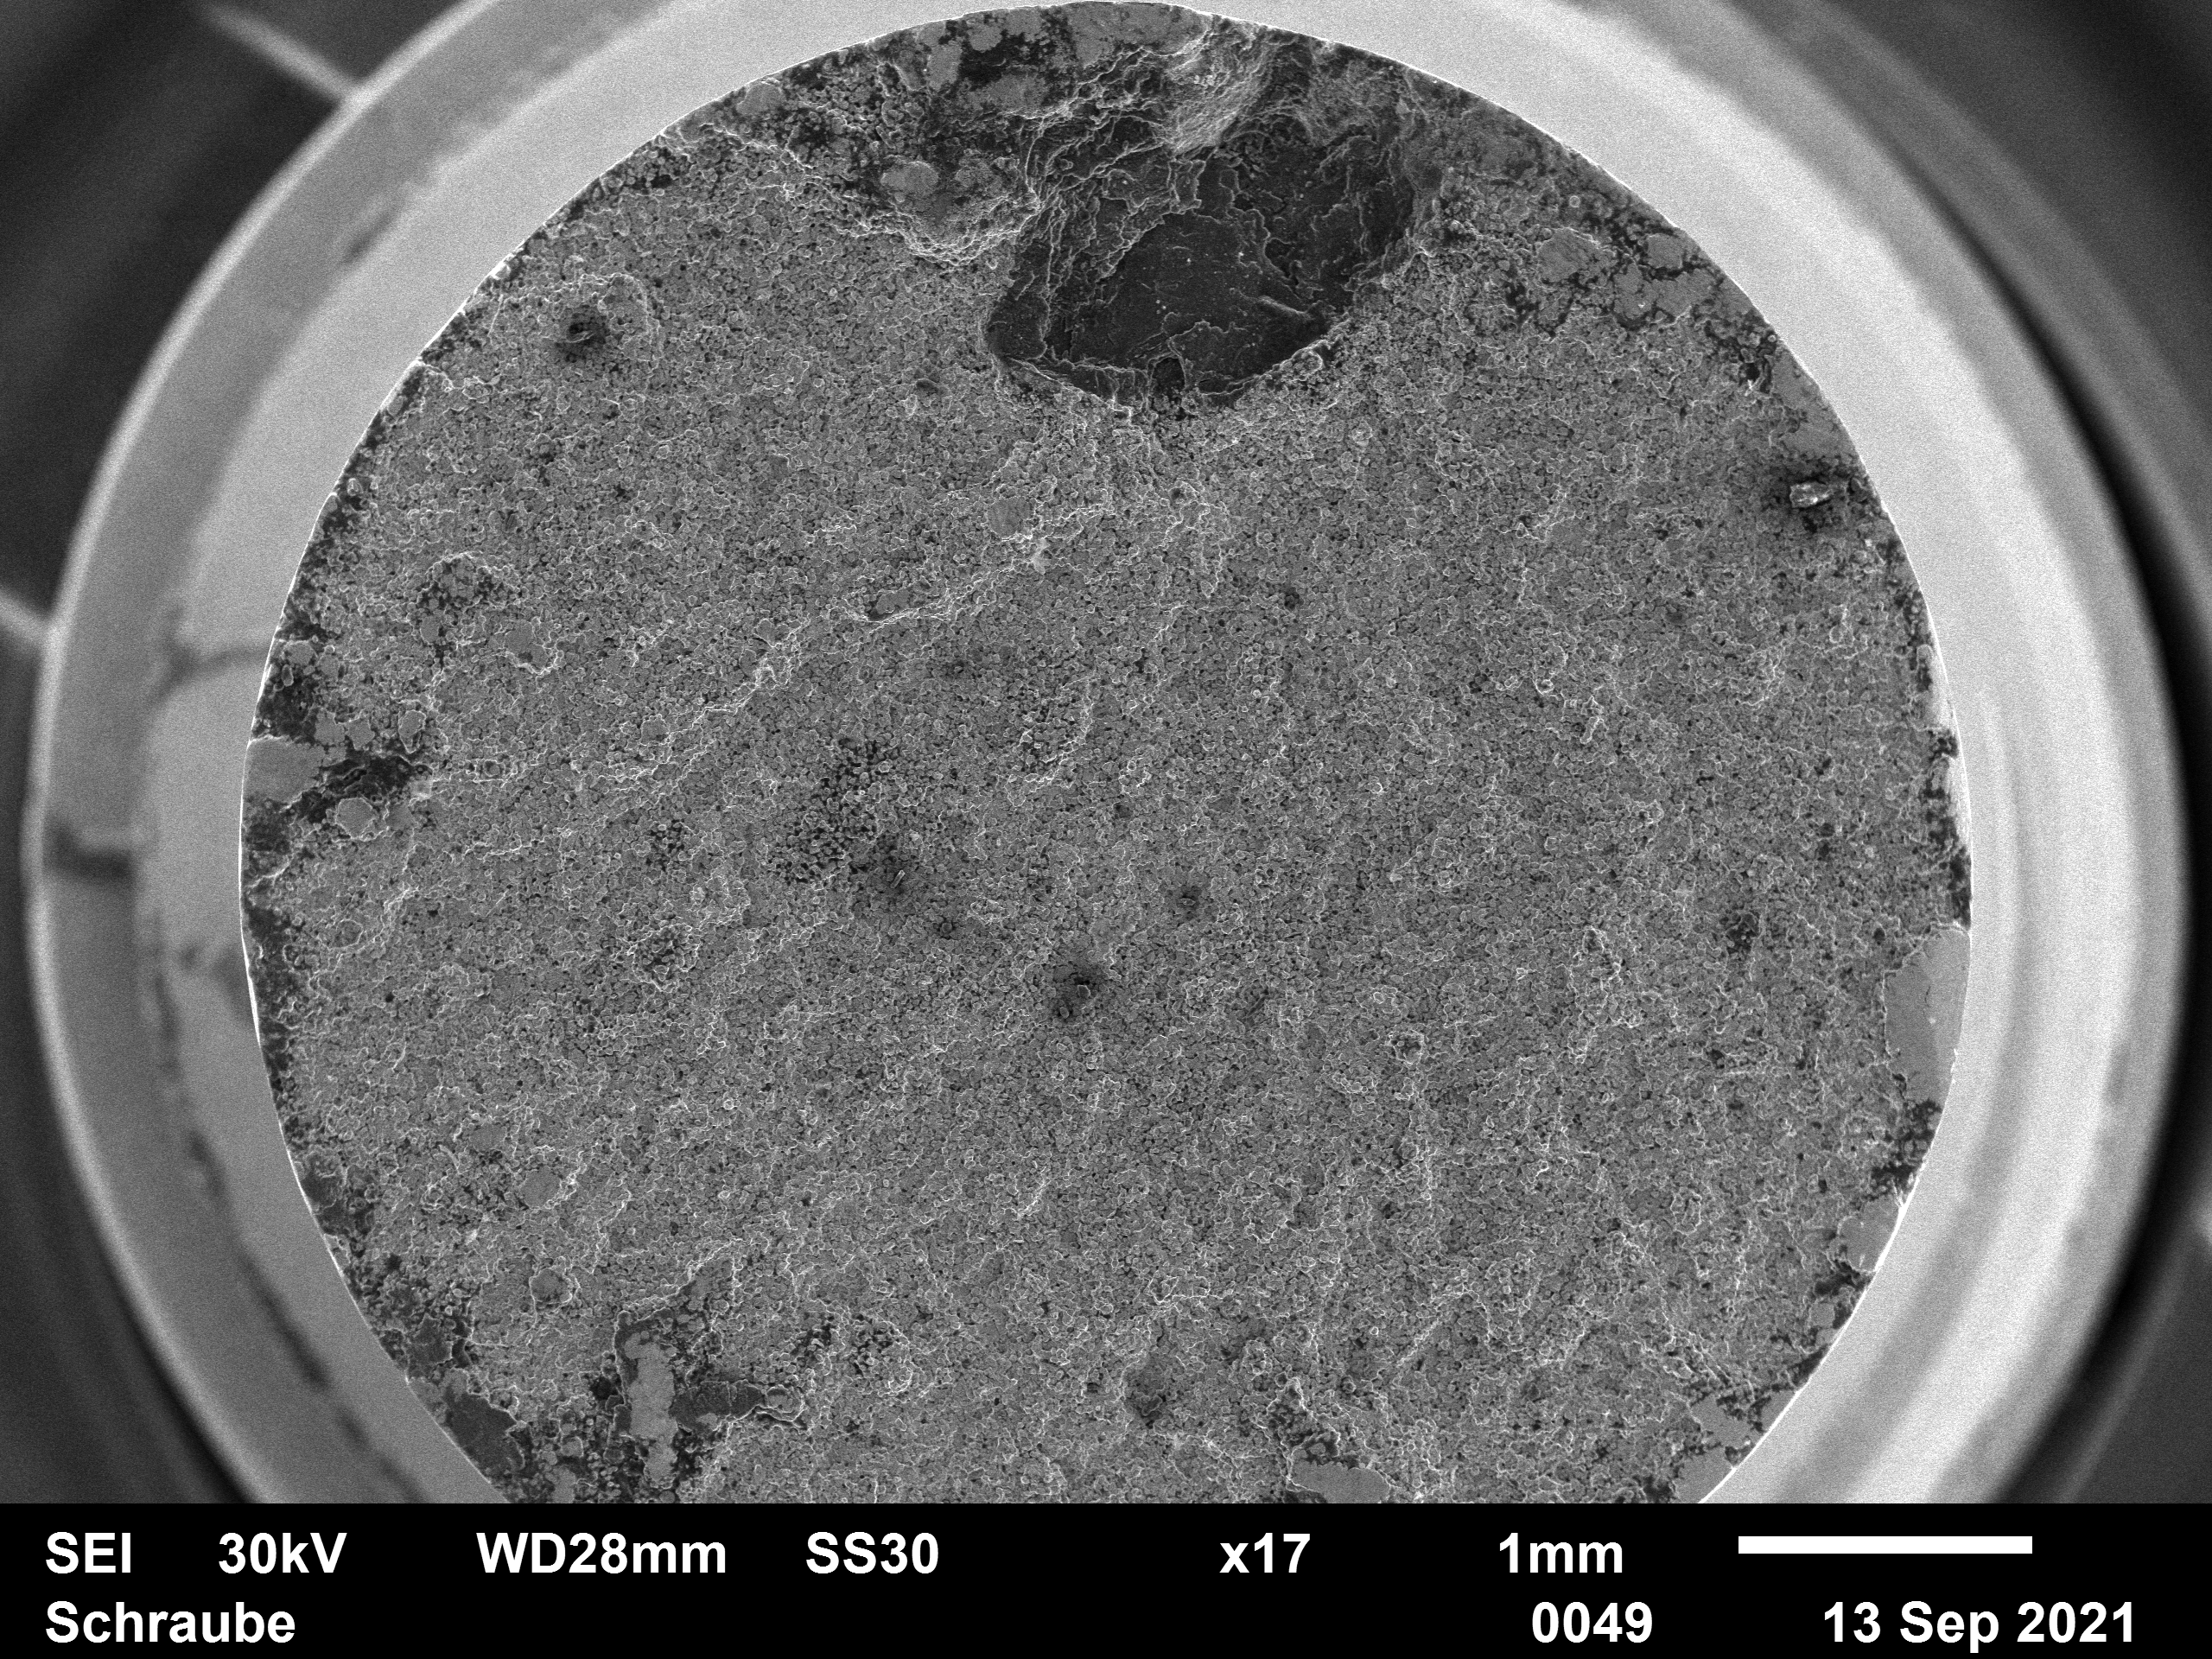
\includegraphics[width=\textwidth]{Auswertung/D/0049.png}
        \caption{SEI}
    \end{subfigure}
    \hfill
    \begin{subfigure}[b]{0.45\textwidth}
        \centering
        \includegraphics[width=\textwidth]{Auswertung/D/0048.png}
        \caption{REF}
    \end{subfigure}
    \\
    \begin{subfigure}[b]{0.45\textwidth}
        \centering
        \includegraphics[width=\textwidth]{Auswertung/D/0047.png}
        \caption{BEC}
    \end{subfigure}
    \caption{Bruchfläche der Schraube mit unterschiedlichen Detektoren}
\end{figure}

Für einen guten ersten Eindruck eignet sich der SEI Modus, um die Struktur der Fläche zu untersuchen, eignet sich der REF Modus. In allen Aufnahmen und besonders im letzten Bild, im BEC Modus, sind drei unterschiedliche Zonen zu erkennen. Zum einen ein recht auffälliger dunkler Fleck im oberen Teil, daneben mehrere kleine hellere Zonen, die sich am Rand der Fläche zu konzentrieren scheinen und der übrige Teil der Schraube, dessen helligkeit zwischen den beiden anderen Zonen liegt. \\

\newpage
Als Nächstes wurde eine Nahaufnahme des dunklen Flecks angefertigt.
\begin{figure}[h]
    \centering
    
    \begin{subfigure}[b]{0.45\textwidth}
        \centering
        \includegraphics[width=\textwidth]{Auswertung/D/0050.png}
        \caption{SEI}
    \end{subfigure}
    \hfill
    \begin{subfigure}[b]{0.45\textwidth}
        \centering
        \includegraphics[width=\textwidth]{Auswertung/D/0051.png}
        \caption{REF}
    \end{subfigure}
    \caption{Nahaufnahme der Kante des dunklen Flecks}
\end{figure}

Aus diesen Aufnahmen geht hervor, dass der dunkle Fleck mit einer Vertiefung einhergeht.

\newpage
Nun soll eine EDX Analyse über die Materialzusammensetzung des dunklen Flecks aufschluss geben.
\begin{figure}[h]
    \centering
    \includegraphics[width=\textwidth]{Auswertung/D/DunkelEDX.png}
    \caption{Röntgenspektrum des dunklen Flecks}
\end{figure}

Markierung der Peaks!\\
Diskussion!\\

\begin{table}[h]
    \centering
    \begin{tabular}{c|c|c|c|c|c|c}
        Element & OZ &Serie& unn. C & norm. C &  Atom. C  & Fehler (1 Sigma) \\
         & & & [Gew. \%] & [Gew. \%] & [At. \%] & [Gew. \%] \\
        \hline\hline
        C & 6 & K & 56,69 & 43,02 & 55,43 & 14,77\\
        O & 8 & K & 41,46 & 31,46 & 30,43 & 10,20\\
        Na & 11 & K & 0,89 & 0,67 & 0,45 & 0,16\\
        Si & 14 & K & 32,74 & 24,85 & 13,69 & 1,56
    \end{tabular}
    \caption{Ergebnisse der EDX-Analyse des dunklen Bereichs}
\end{table}

\newpage
Des Weiteren zeigt eine Nahaufnahmeder hellen gegenden, dass sich diese durch eine gewisse Erhabenheit auszeichnen. Außerdem erscheint die Oberfläche in diesem Bereich ebener.
\begin{figure}[h]
    \centering
    \includegraphics[width=\textwidth]{Auswertung/D/0055.png}
    \caption{Nahaufnahme einer hellen Region}
\end{figure}

\newpage
Über die Zusammensetzung soll wiederum eine EDX Analyse Aufschluss geben.
\begin{figure}[h]
    \centering
    \includegraphics[width=\textwidth]{Auswertung/D/HellEDX.png}
    \caption{Röntgenspektrum der hellen Bereiche}
\end{figure}

Markierung der Peaks!\\
Diskussion!\\

\begin{table}[h]
    \centering
    \begin{tabular}{c|c|c|c|c|c|c}
        Element & OZ &Serie& unn. C & norm. C &  Atom. C  & Fehler (1 Sigma) \\
         & & & [Gew. \%] & [Gew. \%] & [At. \%] & [Gew. \%] \\
        \hline\hline
        C & 6 & K & 18,02 & 16,52 & 52,93 & 5,99\\
        O & 8 & K & 14,29 & 13,10 & 31,51 & 4,47\\
        Fe & 26 & K & 0,57 & 0,53 & 0,36 & 0,08\\
        Ni & 28 & K & 1,38 & 1,27 & 0,83 & 0,12\\
        W & 74 & L & 74,81 & 68,59 & 14,36 & 2,09
    \end{tabular}
    \caption{Ergebnisse der EDX-Analyse der hellen Bereiche}
\end{table}

\newpage
Nicht zu vergessen ist das Grundmaterial der Schraube, auch hierbei wird wieder eine EDX Analyse benutzt.
\begin{figure}[h]
    \centering
    \includegraphics[width=\textwidth]{Auswertung/D/NormalEDX.png}
    \caption{Röntgenspektrum der normalen Bereiche}
\end{figure}

Markierung der Peaks!\\
Diskussion!\\

\begin{table}[h]
    \centering
    \begin{tabular}{c|c|c|c|c|c|c}
        Element & OZ &Serie& unn. C & norm. C &  Atom. C  & Fehler (1 Sigma) \\
         & & & [Gew. \%] & [Gew. \%] & [At. \%] & [Gew. \%] \\
        \hline\hline
        C & 6 & K & 42,64 & 43,61 & 78,17 & 9,71\\
        O & 8 & K & 9,86 & 10,08 & 13,57 & 3,42\\
        Fe & 26 & K & 3,94 & 4,03 & 1,55 & 0,20\\
        Ni & 28 & K & 6,88 & 7,04 & 2,58 & 0,28\\
        W & 74 & L & 34,45 & 35,24 & 4,13 & 1,08
    \end{tabular}
    \caption{Ergebnisse der EDX-Analyse der normalen Bereiche}
\end{table}

Diskussion! Bruchuhrsachenbestimmung!

\newpage
\section{Chip Wafer}